\documentclass[final,acmlarge,draft=false,review=false,nonacm=false]{acmart} 
\usepackage[
    type={CC},              % your choice
    modifier={by-sa},   % your choice
    version={4.0},         % your choice
]{doclicense}               % your choice, see \doclicenseThis below

\settopmatter{printacmref=false,printfolios=false}
\fancyfoot{}

\makeatletter
\def\@formatdoi#1{}
\def\@permissionCodeOne{miniKanren.org/workshop}
\def\@copyrightpermission{\doclicenseThis} % your choice of text
\def\@copyrightowner{Copyright held by the author(s).} % your choice
\makeatother

\copyrightyear{2020}
\setcopyright{rightsretained}

\acmConference[miniKanren 2020]{The Second miniKanren and Relational Programming Workshop}{August 27 2020}{Online}

\acmMonth{8}
\acmArticle{6} % your number in the order of presentations (between 1 and 11)


%% Bibliography style
\bibliographystyle{ACM-Reference-Format}
%% Citation style
%% Note: author/year citations are required for papers published as an
%% issue of PACMPL.
\citestyle{acmauthoryear}   %% For author/year citations


%%%%%%%%%%%%%%%%%%%%%%%%%%%%%%%%%%%%%%%%%%%%%%%%%%%%%%%%%%%%%%%%%%%%%%
%% Note: Authors migrating a paper from PACMPL format to traditional
%% SIGPLAN proceedings format must update the '\documentclass' and
%% topmatter commands above; see 'acmart-sigplanproc-template.tex'.
%%%%%%%%%%%%%%%%%%%%%%%%%%%%%%%%%%%%%%%%%%%%%%%%%%%%%%%%%%%%%%%%%%%%%%


%% Some recommended packages.
\usepackage{booktabs}   %% For formal tables:
                        %% http://ctan.org/pkg/booktabs
\usepackage{subcaption} %% For complex figures with subfigures/subcaptions
                        %% http://ctan.org/pkg/subcaption


\usepackage{amsmath,amssymb}
\usepackage[russian,english]{babel}
\usepackage{amssymb}
\usepackage{mathtools}
\usepackage{listings}
\usepackage{comment}
\usepackage{indentfirst}
\usepackage{hyperref}
\usepackage{amsthm}
\usepackage{stmaryrd}
\usepackage{eufrak}
\usepackage{lstcoq}

\newtheorem{theorem}{Theorem}
\newtheorem{lemma}{Lemma}
\newtheorem{corollary}{Corollary}
\newtheorem{hyp}{Hypethesis}
\newtheorem{definition}{Definition}

\lstdefinelanguage{minikanren}{
keywords={fresh},
sensitive=true,
commentstyle=\small\itshape\ttfamily,
keywordstyle=\textbf,
identifierstyle=\ttfamily,
basewidth={0.5em,0.5em},
columns=fixed,
fontadjust=true,
literate={fun}{{$\lambda\;\;$}}1 {->}{{$\to$}}3 {===}{{$\,\equiv\,$}}1 {=/=}{{$\not\equiv$}}1 {|>}{{$\triangleright$}}3 {/\\}{{$\wedge$}}2 {\\/}{{$\vee$}}2,
morecomment=[s]{(*}{*)}
}

\lstset{
mathescape=true,
language=minikanren
}

\usepackage{letltxmacro}
\newcommand*{\SavedLstInline}{}
\LetLtxMacro\SavedLstInline\lstinline
\DeclareRobustCommand*{\lstinline}{%
  \ifmmode
    \let\SavedBGroup\bgroup
    \def\bgroup{%
      \let\bgroup\SavedBGroup
      \hbox\bgroup
    }%
  \fi
  \SavedLstInline
}

\def\transarrow{\xrightarrow}
\newcommand{\setarrow}[1]{\def\transarrow{#1}}

\def\padding{\phantom{X}}
\newcommand{\setpadding}[1]{\def\padding{#1}}

\def\subarrow{}
\newcommand{\setsubarrow}[1]{\def\subarrow{#1}}

\newcommand{\trule}[2]{\frac{#1}{#2}}
\newcommand{\crule}[3]{\frac{#1}{#2},\;{#3}}
\newcommand{\withenv}[2]{{#1}\vdash{#2}}
\newcommand{\trans}[3]{{#1}\transarrow{\padding{\textstyle #2}\padding}\subarrow{#3}}
\newcommand{\ctrans}[4]{{#1}\transarrow{\padding#2\padding}\subarrow{#3},\;{#4}}
\newcommand{\llang}[1]{\mbox{\lstinline[mathescape]|#1|}}
\newcommand{\pair}[2]{\inbr{{#1}\mid{#2}}}
\newcommand{\inbr}[1]{\left<{#1}\right>}
\newcommand{\highlight}[1]{\color{red}{#1}}
%\newcommand{\ruleno}[1]{\eqno[\scriptsize\textsc{#1}]}
\newcommand{\ruleno}[1]{\mbox{[\textsc{#1}]}}
\newcommand{\rulename}[1]{\textsc{#1}}
\newcommand{\inmath}[1]{\mbox{$#1$}}
\newcommand{\lfp}[1]{fix_{#1}}
\newcommand{\gfp}[1]{Fix_{#1}}
\newcommand{\vsep}{\vspace{-2mm}}
\newcommand{\supp}[1]{\scriptsize{#1}}
\newcommand{\sembr}[1]{\llbracket{#1}\rrbracket}
\newcommand{\cd}[1]{\texttt{#1}}
\newcommand{\free}[1]{\boxed{#1}}
\newcommand{\binds}{\;\mapsto\;}
\newcommand{\dbi}[1]{\mbox{\bf{#1}}}
\newcommand{\sv}[1]{\mbox{\textbf{#1}}}
\newcommand{\bnd}[2]{{#1}\mkern-9mu\binds\mkern-9mu{#2}}
\newcommand{\meta}[1]{{\mathcal{#1}}}
\newcommand{\dom}[1]{\mathtt{dom}\;{#1}}
\newcommand{\primi}[2]{\mathbf{#1}\;{#2}}
\renewcommand{\dom}[1]{\mathcal{D}om\,({#1})}
\newcommand{\ran}[1]{\mathcal{VR}an\,({#1})}
\newcommand{\fv}[1]{\mathcal{FV}\,({#1})}
\newcommand{\tr}[1]{\mathcal{T}r_{#1}}
\newcommand{\diseq}{\not\equiv}
\newcommand{\reprfunset}{\mathcal{R}}
\newcommand{\reprfun}{\mathfrak{f}}
\newcommand{\cstore}{\Omega}
\newcommand{\cstoreinit}{\cstore_\epsilon^{\mathit{init}}}
\newcommand{\csadd}[3]{\mathbf{add}\,(#1, #2 \diseq #3)}  %{#1 + [#2 \diseq #3]}
\newcommand{\csupdate}[2]{\mathbf{update}\,(#1, #2)}  %{#1 \cdot #2}
\newcommand{\cupdate}[2]{\mathbf{update_{constr}}\,(#1, #2)}  %{#1 \cdot #2}
\newcommand{\eqrestr}{=_n}

\newcommand{\searchRule}[6] {
  #1, #2 \vdash (#3, #4) \xRightarrow{#5} #6}
\newcommand{\extSearchRule}[8] {
  #1, #2, #3, #4 \vdash (#5, #6) \xRightarrow{#7}_{e} #8}
\newcommand{\q}{\hspace{0.5em}}
\newcommand{\bigcdot}{\boldsymbol{\cdot}}
\newcommand{\bigslant}[2]{{\raisebox{.2em}{$#1$}\left/\raisebox{-.2em}{$#2$}\right.}}

\let\emptyset\varnothing
\let\eps\varepsilon

\sloppy

\begin{document}

%% Title information
\title{Certified Semantics for Disequality} %% [Short Title] is optional;
                                           %% when present, will be used in
                                           %% header instead of Full Title.
\titlenote{The reported study was funded by RFBR, project number 18-01-00380} %% \titlenote is optional;
                                        %% can be repeated if necessary;
                                        %% contents suppressed with 'anonymous'
%\subtitle{Subtitle}                     %% \subtitle is optional
%\subtitlenote{with subtitle note}       %% \subtitlenote is optional;
                                        %% can be repeated if necessary;
                                        %% contents suppressed with 'anonymous'


%% Author information
%% Contents and number of authors suppressed with 'anonymous'.
%% Each author should be introduced by \author, followed by
%% \authornote (optional), \orcid (optional), \affiliation, and
%% \email.
%% An author may have multiple affiliations and/or emails; repeat the
%% appropriate command.
%% Many elements are not rendered, but should be provided for metadata
%% extraction tools.

\author{Dmitry Rozplokhas}
\affiliation{%
  \institution{Higher School of Economics}, \institution{JetBrains Research}
  \country{Russia}}
\email{rozplokhas@gmail.com}

\author{Dmitry Boulytchev}
\affiliation{%
  \institution{Saint Petersburg State University}, \institution{JetBrains Research}
  \country{Russia}}
\email{dboulytchev@math.spbu.ru}



%% Abstract
%% Note: \begin{abstract}...\end{abstract} environment must come
%% before \maketitle command
\begin{abstract}
We present an extension of our prior work on certified semantics for core \textsc{miniKanren}, introducing disequality constraints in the language.
Semantics is parameterized by an exact definition of constraint stores, allowing us to cover different implementations, and we provide a list of sufficient conditions on this definition for search completeness.
We also give two examples of concrete implementations of constraint stores that satisfy those sufficient conditions.
The description and proofs for parameterized semantics and both implementations are certified in Coq and two correct-by-construction interpreters are extracted.
\end{abstract}


%% 2012 ACM Computing Classification System (CSS) concepts
%% Generate at 'http://dl.acm.org/ccs/ccs.cfm'.
\begin{CCSXML}
<ccs2012>
<concept>
<concept_id>10003752.10003790.10003795</concept_id>
<concept_desc>Theory of computation~Constraint and logic programming</concept_desc>
<concept_significance>500</concept_significance>
</concept>
<concept>
<concept_id>10003752.10010124.10010131.10010133</concept_id>
<concept_desc>Theory of computation~Denotational semantics</concept_desc>
<concept_significance>500</concept_significance>
</concept>
<concept>
<concept_id>10003752.10010124.10010131.10010134</concept_id>
<concept_desc>Theory of computation~Operational semantics</concept_desc>
<concept_significance>500</concept_significance>
</concept>
</ccs2012>
\end{CCSXML}
%% \ccsdesc[500]{Theory of computation~Constraint and logic programming}
%% \ccsdesc[500]{Theory of computation~Denotational semantics}
%% \ccsdesc[500]{Theory of computation~Operational semantics}
%% End of generated code


%% Keywords
%% comma separated list
%% \keywords{Relational programming, denotational semantics, operational semantics, certified programming}  %% \keywords are mandatory in final camera-ready submission


%% \maketitle
%% Note: \maketitle command must come after title commands, author
%% commands, abstract environment, Computing Classification System
%% environment and commands, and keywords command.
\maketitle
\thispagestyle{empty}

\section{Introduction}
\label{sec:intro}

This paper deals with the problem of the worst-case time complexity estimations for relational program evaluation in the canonical implementation of \mK based on interleaving search~\cite{TRS}. Despite its simple implementation, the search in \mK has a number of subtleties
affecting the performance, which are hard to think about intuitively altogether. It is easy to overlook some of them and the behavior of the search in certain cases can be really surprising.

\begin{figure}[t]
\begin{tabular}{p{5cm}p{5cm}}
\begin{lstlisting}[basicstyle=\small]
   length$^o$ = fun a n ->
     ((a === Nil) /\ (n === O)) \/
     (fresh (h t n')
        (a === Cons(h, t)) /\
        (n === S(n')) /\
        (length$^o$ t n'))
     )
\end{lstlisting} &
\begin{lstlisting}[basicstyle=\small]
   length$_d^o$ = fun a n ->
     ((a === Nil) /\ (n === O)) \/
     (fresh (h t n')
        (a === Cons(h, t)) /\
        (length$_d^o$ t n') /\
        (n === S(n')))
     )
\end{lstlisting}
\end{tabular}
\caption{Example of two implementations of the length calculating relation}
\label{fig:length_implementations}
\end{figure}

\begin{figure}[t]
    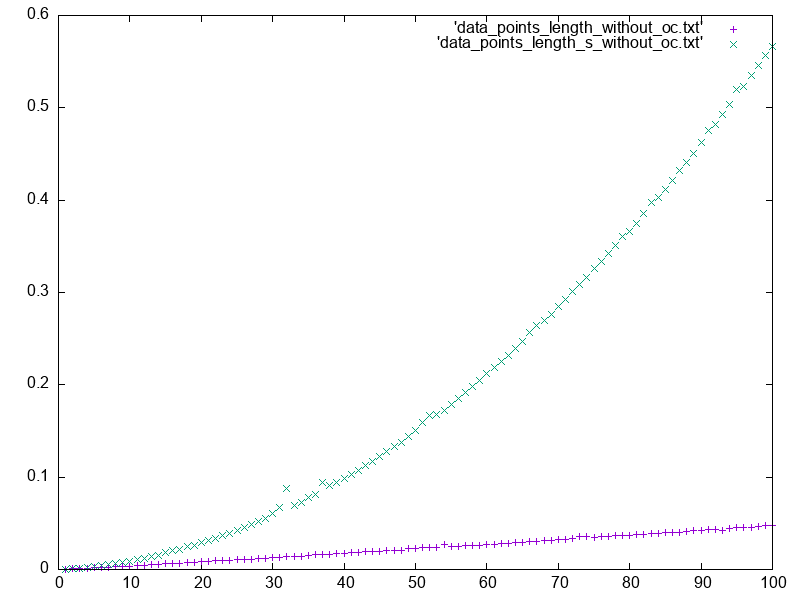
\includegraphics[width=6cm,height=5cm]{lengths_without_oc.png}
    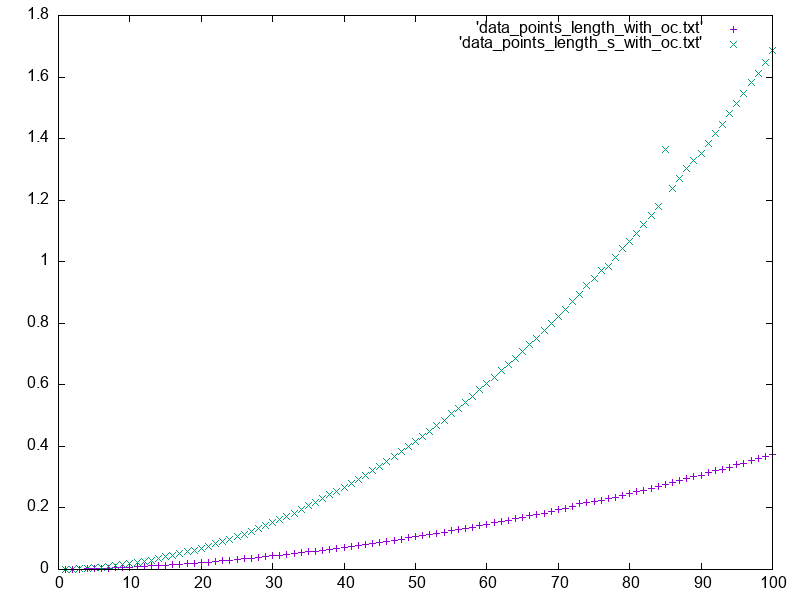
\includegraphics[width=6cm,height=5cm]{lengths_with_oc.png}
  \caption{Time (in seconds) of the search for the relations \lstinline|length$^o$| (purple) and \lstinline|length$_d^o$|} (green) depending on the lentgh of the list.
  Left: without occurs check.
  Right: with occurs check.
  \label{fig:length_plots}
\end{figure}

As a motivative example, consider two implementations of a standard recursive relation calculating the length of a list (see \figureword~\ref{fig:length_implementations}). They differ only in the
orders of conjuncts. Although the \lstinline|length$_d^o$| relation can be seen as a more direct definition of a function as a relation (all steps of usual length evaluation written up in order),
it is well-known that the \lstinline|length$^o$| with the recursive call in the end is much faster when running this relation backward (in fact, the search diverges if we
run \lstinline|length$_d^o$| backward, while for \lstinline|length$^o$| it terminates). What is less known and what we find more unexpected is the fact that if we run both relations
forward (specifying the list and asking for the length) \lstinline|length$^o$| is still much faster than \lstinline|length$_d^o$|, although they perform the same number of unifications. You can see the comparative time of the search in \figureword~\ref{fig:length_plots}. The difference is even
more staggering if we switch off occurs checks in unifications. It's OK because for simple queries like this occurs checks never violated. In the same \figureword~\ref{fig:length_plots} you can see that
the \emph{asymptotic complexity} becomes different in this case: it is linear for \lstinline|length$^o$| and quadratic for \lstinline|length$_d^o$|.

After investigating the execution for this example in detail we found that the difference is caused not by unifications but by the process of \emph{scheduling} of goals during the search.
During the execution of a program in \mK a lazy structure is build that decomposes the goals into unifications, performs these unifications in a certain order, and passes the results
appropriately. For the \lstinline|length$_d^o$| relation this structure becomes linear in size just because of the order in conjunctions and increases the time of
scheduling significantly. This kind of effect is hard to predict and measure without a formal model for performance in \mK.

This paper presents such a model. We study evaluation in a specific (canonical) implementation of \mK with goals evaluated to lazy streams in program-written order, but we rely only on the basic principles of implementation of \mK, so the model should be easily addoptable for a large class of regular implementations. We state that the total time of the search in \mK breaks into three separate parts: the time of scheduling ($T_s$) that breaks the evaluation into a sequence of
unifications, the time required to perform these unifications, and the time of reifications ($T_r$) that reconstruct the result in an expected form in the end. The time of unifications can be further
divided into the time of occurs checks ($T_{occ}$) during the unification and the time ($T_{uni}$) of the rest of the unification algorithm (this division will help us to see how large
is the part of the total time that occurs check, which often can be omitted, takes). So the total time of the search can be calculated as the sum of four components:

\[ T = T_s + T_{uni} + T_{occ} + T_r \]

We show how these components can be estimated and compared to each other in terms of asymptotics. The scheduling time complexity can be measured precisely since we link it to a specific value which we
call \emph{scheduling factor}, defined in terms of existing formal semantics of \mK (we recall the existing formal descriptions of \mK in \sectionword~\ref{sec:background}) and can be calculated using
a number of equations (\sectionword~\ref{sec:scheduling}). The other time components are hard to estimate precisely in general, as they are connected to the unification process, but we identify two
criteria that determine a wide range of cases for which these time components can be estimated easily (\sectionword~\ref{sec:uni-rei}). These separate methods for estimation of
different components of the time of the search can be put together in one approach for calculating manually the time complexity for a given query to a recursive relation (if this query satisfies the stated
criteria) using the principles of symbolic execution (\sectionword~\ref{sec:symbolic}). We then show the applicability of our method by applying it for a number of realistic \mK relations (\sectionword~\ref{sec:evaluation}).

\section{The syntax and semantics of the core language}
\label{sec:review}

In this section, we recall existing definitions of the syntax and the two semantics for the core language without disequality constraints and the main result~--- the equivalence
of these two semantics~\cite{CertifiedSemantics}.

\subsection{The Syntax of Core Language}
\label{subsec_syntax}

\begin{figure}[t]
\centering
\[
\begin{array}{ccll}
  \mathcal{C} & = & \{C_i^{k_i}\} & \mbox{constructors with arities} \\
  \mathcal{T}_X & = & X \cup \{C_i^{k_i} (t_1, \dots, t_{k_i}) \mid t_j\in\mathcal{T}_X\} & \mbox{terms over the set of variables $X$} \\
  \mathcal{D} & = & \mathcal{T}_\emptyset & \mbox{ground terms}\\
  \mathcal{X} & = & \{ x, y, z, \dots \} & \mbox{syntactic variables} \\
  \mathcal{A} & = & \{ \alpha, \beta, \gamma, \dots \} & \mbox{semantic variables} \\
  \mathcal{R} & = & \{ R_i^{k_i}\} &\mbox{relational symbols with arities} \\[2mm]
  \mathcal{G} & = & \mathcal{T_X}\equiv\mathcal{T_X}   &  \mbox{equality} \\
              &   & \mathcal{G}\wedge\mathcal{G}     & \mbox{conjunction} \\
              &   & \mathcal{G}\vee\mathcal{G}       &\mbox{disjunction} \\
              &   & \mbox{\lstinline|fresh|}\;\mathcal{X}\;.\;\mathcal{G} & \mbox{fresh variable introduction} \\
              &   & R_i^{k_i} (t_1,\dots,t_{k_i}),\;t_j\in\mathcal{T_X} & \mbox{relational symbol invocation} \\[2mm]
  \mathcal{S} & = & \{R_i^{k_i} = \lambda\;x_1^i\dots x_{k_i}^i\,.\, g_i;\}\; g & \mbox{specification}
\end{array}
\]
\caption{The syntax of core language}
\label{syntax}
\end{figure}

The syntax of the language is shown in Fig.~\ref{syntax}. First, we fix a set of constructors $\mathcal{C}$ with known arities and consider
a set of terms $\mathcal{T}_X$ with constructors as functional symbols and variables from $X$. We parameterize this set with an alphabet of
variables since in the semantic description we will need \emph{two} kinds of variables. The first kind, \emph{syntactic} variables, is denoted
by $\mathcal{X}$. We also consider an alphabet of \emph{relational symbols} $\mathcal{R}$ which are used to name relational definitions.
The central syntactic category in the language is a \emph{goal}. In our case, there are five types of goals: \emph{equality} of terms,
conjunction and disjunction of goals, fresh variable introduction, and invocation of some relational definition. Thus, equality is used
as a constraint, and multiple constraints can be combined using conjunction, disjunction, and recursion. For the sake of brevity we
abbreviate immediately nested ``\lstinline|fresh|'' constructs into the one, writing ``\lstinline|fresh $x$ $y$ $\dots$ . $g$|'' instead of
``\lstinline|fresh $x$ . fresh $y$ . $\dots$ $g$|''. The final syntactic category is \emph{specification} $\mathcal{S}$. It consists of a set
of relational definitions and a top-level goal. A top-level goal represents a search procedure which returns a stream of substitutions for
the free variables of the goal. The language we defined is first-order, as goals can not be passed as parameters,
returned or constructed at runtime.

As an example consider the specification for the standard \lstinline|append$^o$| relation and a query which splits a list containing
three constants \lstinline|A|, \lstinline|B| and \lstinline|C| into two parts in every possible way:

\begin{minipage}{\linewidth}
\begin{lstlisting}
  append$^o$ = fun x y xy .
    ((x === Nil) /\ (xy === y)) \/
    (fresh h t ty .
       (x  === Cons (h, t))  /\
       (xy === Cons (h, ty)) /\
       (append$^o$ t y ty)
    );
  append$^o$ x y (Cons (A, Cons (B, Cons (C, Nil))))
\end{lstlisting}
\end{minipage}

\subsection{Denotational sematics}

For denotational semantics, we use a simple set-theoretic approach which can be considered analogous to the least Herbrand model for definite logic programs~\cite{LHM}.

Intuitively, the mathematical model for every goal should be a relation between semantic variables that occur free in this goal. We represent this relation as a set of total
functions 

\[
\mathfrak{f}:\mathcal{A}\mapsto\mathcal{D}
\]

from semantic variables to ground terms. We call these functions \emph{representing functions}.

Then, the semantic function for goals is parameterized over environments which prescribe semantic functions to relational symbols:

\[
  \Gamma : \mathcal{R} \to (\mathcal{T_A}^*\to 2^{\mathcal{A}\to\mathcal{D}})
\]

An environment associates with relational symbol a function that takes a string of terms (the arguments of the relation) and returns a set of
representing functions. The signature for semantic brackets for goals is as follows:

\[
\sembr{\bullet}_{\Gamma} : \mathcal{G}\to 2^{\mathcal{A}\to\mathcal{D}}
\]

It maps a goal into the set of representing functions w.r.t. an environment $\Gamma$.

We formulate the following important \emph{completeness condition} for the semantics of a goal $g$: for any goal $g$ and two representing functions ${\mathfrak f}$ and ${\mathfrak f'}$, such that $\left.{\mathfrak f}\right|_{FV(g)} = \left.{\mathfrak f'}\right|_{FV(g)}$
\[ {\mathfrak f} \in \sembr{g} \Leftrightarrow {\mathfrak f'} \in \sembr{g} \]

In other words, representing functions for a goal $g$ restrict only the values of free variables of $g$ and do not introduce any ``hidden'' correlations.
This condition guarantees that our semantics is complete in the sense that it does not introduce artificial restrictions for the relation it defines.
We proved that the semantics of goals always satisfy this condition.

To define the semantic function we need a few operations for representing functions:

\begin{itemize}
\item A homomorphic extension of a representing function 

\[
  \overline{\mathfrak{f}}:\mathcal{T_A}\to\mathcal{D}
\]

which maps terms to terms:

\[
\begin{array}{rcl}

  \overline{\mathfrak f}\,(\alpha) & = & \mathfrak f\,(\alpha)\\
  \overline{\mathfrak f}\,(C_i^{k_i}\,(t_1,\dots.t_{k_i})) & = & C_i^{k_i}\,(\overline{\mathfrak f}\,(t_1),\dots \overline{\mathfrak f}\,(t_{k_i}))
\end{array}
\]

\item A pointwise modification of a function

\[
f\,[x\gets v]\,(z)=\left\{
\begin{array}{rcl}
  f\,(z) &,& z \ne x \\
  v      &,& z = x
\end{array}
\right.
\]

\item A \emph{generalization} operation:

\[
\mathfrak{f}\uparrow\alpha = \{ \mathfrak{f}\,[\alpha\gets d] \mid d\in\mathcal D\}
\]

Informally, this operation generalizes a representing function into a set of representing functions in such a way that the
values of these functions for a given variable cover the whole $\mathcal{D}$. We extend the generalization operation for sets of
representing functions $\mathfrak{F}\subseteq\mathcal{A}\to\mathcal{D}$:

\[
  \mathfrak{F}\uparrow\alpha = \bigcup_{\mathfrak{f}\in\mathfrak{F}}(\mathfrak{f}\uparrow\alpha)
\]

\end{itemize}

The semantics for goals is shown on Fig.~\ref{denotational_semantics_of_goals}.

\begin{figure}[t]
  \[
  \begin{array}{cclr}
    \sembr{t_1\equiv t_2}_\Gamma&=&\{\mathfrak f : \mathcal{A}\to\mathcal{D}\mid \overline{\mathfrak{f}}\,(t_1)=\overline{\mathfrak{f}}\,(t_2)\}& \ruleno{Unify$_D$}\\
    \sembr{g_1\wedge g_2}_\Gamma&=&\sembr{g_1}_\Gamma\cap\sembr{g_1}_\Gamma&\ruleno{Conj$_D$}\\
    \sembr{g_1\vee g_2}_\Gamma&=&\sembr{g_1}_\Gamma\cup\sembr{g_1}_\Gamma&\ruleno{Disj$_D$}\\
    \sembr{\mbox{\lstinline|fresh|}\,x\,.\,g}_\Gamma&=&(\sembr{g\,[\alpha/x]}_\Gamma)\uparrow\alpha,\;\alpha\not\in FV(g)& \ruleno{Fresh$_D$}\\
    \sembr{R\,(t_1,\dots,t_k)}_\Gamma&=&(\Gamma\,R)\,t_1\dots t_k & \ruleno{Invoke$_D$}
  \end{array}
  \]
  \caption{Denotational semantics of goals}
  \label{denotational_semantics_of_goals}
\end{figure}

The final component is the semantics of specifications. Given a specification

\[
\{R_i=\lambda\,x_1^i\dots x_{k_i}^i\,.\,g_i;\}_{i=1}^n\;g
\]

we construct a correct environment $\Gamma_0$ and then take the semantics of the top-level goal:

\[
\sembr{\{R_i=\lambda\,x_1^i\dots x_{k_i}^i\,.\,g_i;\}_{i=1}^n\;g}=\sembr{g}_{\Gamma_0}
\]

As the set of definitions can be mutually recursive we apply the fixed point approach and define $\Gamma_0$ as the least
fixed point of a specific function $F$ that takes an environment $\Gamma$ and returns new environment in which semantics
of a body of each definition is evaluated with environment $\Gamma$.


\subsection{Operational sematics}

The operational semantics of \textsc{miniKanren}, which we described, corresponds to the known
implementations with interleaving search. The semantics is given in the form of a labeled transition system (LTS)~\cite{LTS}.

The states in the transition system have the following shape:

\[
S = \mathcal{G}\times\Sigma\times\mathbb{N}\mid S\oplus S \mid S \otimes \mathcal{G}
\]

A state has a tree-like structure with intermediate nodes corresponding to partially-evaluated conjunctions (``$\otimes$'') or
disjunctions (``$\oplus$''). A leaf in the form $\inbr{g, \sigma, n}$ determines a goal in a context, where $g$~--- a goal, $\sigma$~--- a substitution accumulated so far,
and $n$~--- a natural number, which corresponds to a number of semantic variables used to this point. For a conjunction node, its right child is always a goal since
it cannot be evaluated unless some result is provided by the left conjunct.

We also need extended states

\[
\overline{S} = \diamond \mid S
\]

where $\diamond$ symbolizes the end of the evaluation.

The set of labels is defined as follows:

\[
L = \circ \mid \Sigma\times \mathbb{N}
\]

The label ``$\circ$'' is used to mark those steps which do not provide an answer; otherwise, a transition is labeled by a pair of a substitution and a number of allocated
variables. The substitution is one of the answers, and the number is threaded through the derivation to keep track of the allocated variables.

\begin{figure*}
  \renewcommand{\arraystretch}{1.6}
  \[
  \begin{array}{cr}
    \inbr{t_1 \equiv t_2, \sigma, n} \xrightarrow{\circ} \Diamond , \, \, \nexists\; mgu\,(t_1 \sigma, t_2 \sigma) &\ruleno{UnifyFail} \\
    \inbr{t_1 \equiv t_2, \sigma, n} \xrightarrow{(mgu\,(t_1 \sigma, t_2 \sigma) \circ \sigma),\, n)} \Diamond & \ruleno{UnifySuccess} \\
    \inbr{g_1 \lor g_2, \sigma, n} \xrightarrow{\circ} \inbr{g_1, \sigma, n} \oplus \inbr{g_2, \sigma, n} & \ruleno{Disj} \\
    \inbr{g_1 \land g_2, \sigma, n} \xrightarrow{\circ} \inbr{ g_1, \sigma, n} \otimes g_2 & \ruleno{Conj} \\
    \inbr{\mbox{\lstinline|fresh|}\, x\, .\, g, \sigma, n} \xrightarrow{\circ} \inbr{g\,[\bigslant{\alpha_{n + 1}}{x}], \sigma, n + 1} & \ruleno{Fresh} \\
    \dfrac{R_i^{k_i}=\lambda\,x_1\dots x_{k_i}\,.\,g}{\inbr{R_i^{k_i}\,(t_1,\dots,t_{k_i}),\sigma,n} \xrightarrow{\circ} \inbr{g\,[\bigslant{t_1}{x_1}\dots\bigslant{t_{k_i}}{x_{k_i}}], \sigma, n}} & \ruleno{Invoke}\\
    \dfrac{s_1 \xrightarrow{\circ} \Diamond}{(s_1 \oplus s_2) \xrightarrow{\circ} s_2} & \ruleno{DisjStop}\\
    \dfrac{s_1 \xrightarrow{r} \Diamond}{(s_1 \oplus s_2) \xrightarrow{r} s_2} & \ruleno{DisjStopAns}\\
    \dfrac{s \xrightarrow{\circ} \Diamond}{(s \otimes g) \xrightarrow{\circ} \Diamond} &\ruleno{ConjStop}\\
    \dfrac{s \xrightarrow{(\sigma, n)} \Diamond}{(s \otimes g) \xrightarrow{\circ} \inbr{g, \sigma, n}}  & \ruleno{ConjStopAns}\\
    \dfrac{s_1 \xrightarrow{\circ} s'_1}{(s_1 \oplus s_2) \xrightarrow{\circ} (s_2 \oplus s'_1)} &\ruleno{DisjStep}\\
    \dfrac{s_1 \xrightarrow{r} s'_1}{(s_1 \oplus s_2) \xrightarrow{r} (s_2 \oplus s'_1)} &\ruleno{DisjStepAns}\\
    \dfrac{s \xrightarrow{\circ} s'}{(s \otimes g) \xrightarrow{\circ} (s' \otimes g)} &\ruleno{ConjStep}\\
    \dfrac{s \xrightarrow{(\sigma, n)} s'}{(s \otimes g) \xrightarrow{\circ} (\inbr{g, \sigma, n} \oplus (s' \otimes g))} & \ruleno{ConjStepAns} 
  \end{array}
  \]
  \caption{Operational semantics of interleaving search}
  \label{lts}
\end{figure*}

The transition rules are shown in Fig.~\ref{lts}. The introduced transition system is completely deterministic.

A derivation sequence for a certain state $s$ determines a \emph{trace} $\tr{s}$~--- a finite or infinite sequence of answers. The trace corresponds to the stream of answers
in the reference \textsc{miniKanren} implementations.

\subsection{Semantics Equivalence}

After we defined two different kinds of semantics for \textsc{miniKanren} we related them and showed that the results given by these two semantics are the same for any specification.
By proving this equivalence we established the \emph{completeness} of the search which means that the search will get all answers satisfying the described specification and only those.

To do it we had to relate the answers produced by these two semantics as they have different forms: a trace of substitutions (along with numbers of allocated variables)
for operational and a set of representing functions for denotational. There is a natural way to extend any substitution to a representing function: composing it with an arbitrary representing function will preserve all variable dependencies in the substitution. So we defined a set of representing functions corresponding to substitution as follows:

\[
\sembr{\sigma} = \{\overline{\mathfrak f} \circ \sigma \mid \mathfrak{f}:\mathcal{A}\mapsto\mathcal{D}\}
\]

And \emph{denotational analog} of an operational semantics (a set of representing functions corresponding to answers in the trace) for given extended state $s$ is
then defined as a union of sets for all substitution in the trace:

\[
\sembr{s}_{op} = \cup_{(\sigma, n) \in \tr{s}} \sembr{\sigma}
\]

This allowed us to state the theorem relating two semantics.

\begin{theorem}[Operational semantics soundness and completeness]
For any specification $\{\dots\}\; g$, for which the indices of all free variables in $g$ are limited by some number $n$

\[
\sembr{\inbr{g, \epsilon, n}}_{op} \eqrestr \sembr{\{\dots\}\; g}.
\]
\end{theorem}

Where `$\eqrestr$' means that we compare representing functions of these sets only on the semantic variables from $\{\alpha_1, \dots, \alpha_n\}$:

\[
S_1 \eqrestr S_2 \xLeftrightarrow{def}  \{\mathfrak{f}|_{\{\alpha_1,\dots,\alpha_n\}} \mid \mathfrak{f} \in S_1 \} = \{\mathfrak{f}|_{\{\alpha_1,\dots,\alpha_n\}} \mid \mathfrak{f} \in S_2 \}.
\]

We can not use the usual equality of sets instead of this one, the sets from the theorem statement are actually not equal.
The reason for this is that denotational semantics encodes only dependencies between the free variables of a goal, which is reflected by the completeness condition, while
operational semantics may also contain dependencies between semantic variables allocated in ``\lstinline|fresh|''.
Therefore we have to restrict representing functions on the semantic variables allocated in the beginning (which includes all free variables of a goal). This does not
compromise our promise to prove the completeness of the search as \textsc{miniKanren} provides the result as substitutions only for queried variables,
which are allocated in the beginning.

The proof of this main theorem was certified in \textsc{Coq}.
\input{extension.tex}
\input{implementations.tex}
\input{applications.tex}
\section{Conclusion}
\label{conclusion}

We presented an improvement of a search strategy for relational programming, which is aimed at
improving refutationally completeness. We've proven, that in the case of a finite number of 
answers our modification is a strict improvement over the original strategy. Our evaluation 
shows, that w.r.t. the improved search many practically important refutationally incomplete 
queries became refutationally complete; in addition in a number of cases the performance was greatly 
improved since our modification, as a side effect, causes the search to choose more 
``optimistic'' branches. 

We can identify the following directions for future work. 

First, we believe, that our result on refutational improvement for a finite number of answers 
can be extended to the general case as well (note, in our current development we did not make 
any use of the \emph{completeness} property of miniKanren search). For this, we would also need 
another, more general, semantics. 

Another direction is extending the language with disequality constraints. Our evaluation has 
shown, that disequality constraints do not compromise our improvement in all user benchmarks, 
but we do not have a proof, that they are indeed harmless.

Next, we are working on a certified proof of the main theorem in Coq.

Finally, our practical evaluation is performed only for a prototype. 
We consider the embedding of our improvement in a full-fledged implementation to be
an important task.

%% Acknowledgments
%\begin{acks}                            %% acks environment is optional
                                        %% contents suppressed with 'anonymous'
  %% Commands \grantsponsor{<sponsorID>}{<name>}{<url>} and
  %% \grantnum[<url>]{<sponsorID>}{<number>} should be used to
  %% acknowledge financial support and will be used by metadata
  %% extraction tools.
 % This material is based upon work supported by the
  %\grantsponsor{GS100000001}{National Science
   % Foundation}{http://dx.doi.org/10.13039/100000001} under Grant
  %No.~\grantnum{GS100000001}{nnnnnnn} and Grant
  %No.~\grantnum{GS100000001}{mmmmmmm}.  Any opinions, findings, and
  %conclusions or recommendations expressed in this material are those
  %of the author and do not necessarily reflect the views of the
  %National Science Foundation.
%\end{acks}


%% Bibliography
\bibliography{main}


%% Appendix
%\appendix
%\section{Appendix}

%Text of appendix \ldots

\end{document}
